\documentclass{home_assignment}
\usepackage{hyperref}
\begin{document}
\titlePage{Monolithic, Service-oriented and Microservices based Architectures}{August 3, 2021}{Basanta Joshi, Ph.D.}
    \pagenumbering{roman}
    \clearpage
    \tableofcontents
    \clearpage
    \phantomsection
    \addcontentsline{toc}{section}{\bfseries{List of Figures}}
    \listoffigures  
    \clearpage
    \phantomsection
    \addcontentsline{toc}{section}{\bfseries{List of Tables}}
    \listoftables  
    \clearpage
    \pagenumbering{arabic}
    \section{Background Theory}
    Software development at a production level is a tough ask, especially with the growing field of technology. There are many software architectures that are used while putting together different components that compose a properly functioning product, out of which this report deals with three of the most popular architectures, viz. Monolithic, service-oriented and Microservices. These architectures are under considerable debate since large companies like Amazon, Netflix, Google have made microservices popular. However, the monolithic and service-oriented architecture aren't outdated, but are rather useful given the correct usage. In this report, we discuss the types of architectures and also compare the three architectures under different key points of consideration.
    \subsection{Monolithic Architecture}
    Monolithic architecture is considered as a primitive way of building applications since the application is built as a single indivisible unit. The applications developed following the monolithic architecture contain a server-side application (business logic), a client-side user interface and a database. All the application functions are managed and served at a single place leading to a larger code base that often lacks modularity. Due to the single larger code base, updates to the application is tedious and lead to the entire stack requiring breaking changes. It is easier in implementation and mostly useful for smaller projects where regular updates isn't all that necessary, rather a faster deployment time is prioritized. As the application developed using a monolithic architecture functions as a single block, issues to any function jeopardizes the entire application. Newer technologies are difficult to implement as the entire application needs to be rewritten. However, there are quite fewer cross-cutting concerns such as rate limiting, audit trails, logging and such. 
\begin{figure}[H]
    \centering
    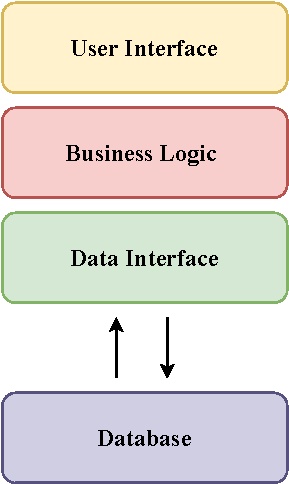
\includegraphics{../Figures/Monolith.pdf}
    \caption{Monolithic architecture}
    \label{fig:mono}
\end{figure}
\subsection{Service-oriented Architecture}
Service-oriented architecture, as the name suggests, is a software architecture that idealizes an application containing discrete software agents that are loosely coupled to perform the required function. It is also known as centralized oriented architecture since multiple user agents are used for interaction with a single central system. Each service provides a different functionality that is properly abstracted creating a self contained black box that reduces overhead. Each service is abstract and hence can be developed using different technology. Enterprise service bus takes care of all services and interacts with each one separately. This means if a single service is faulty, the entire application is jeopardized and hence a better fault tolerance is achieved. Similarly, service reusability is possible with this architecture. However, the enterprise service bus becomes the single point of failure and may cause the entire application to collapse if it fails.
\begin{figure}[H]
    \centering
    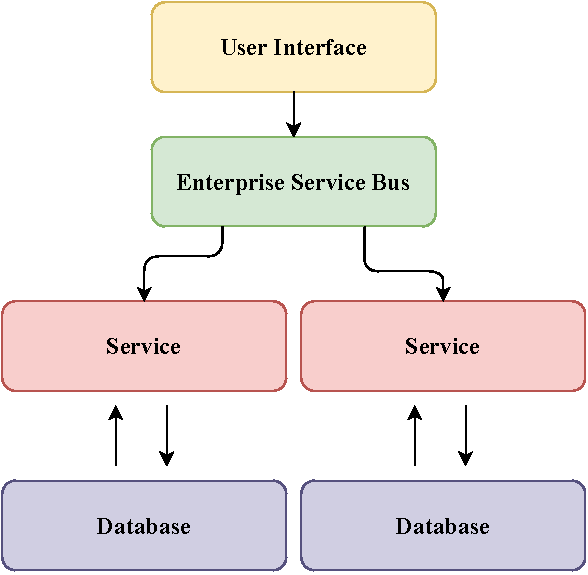
\includegraphics{../Figures/soa.pdf}
    \caption{Service-oriented architecture}
    \label{fig:soa}
\end{figure}
\subsection{Microservices Architecture}
Microservice architecture is a form of service-oriented software architecture that idealizes on building autonomous components that compose an application. Microservice applications consist of multiple independent components that function together with application programming interfaces (APIs). A key difference from the service-oriented architecture is that it is not connected to a central service, rather all the different components are self-contained and autonomous. For communication among such components, the applications make use of APIs that is somewhat a complex task, but provides maximum fault tolerance to application failures due to service damage. It provides better scalability and updates to the application are easier. The code base is modular and bug detection and troubleshooting is easier as a component doesn't affect any other service. Cross-cutting concerns are essential for applications using microservices architecture. Complexity and difficulty in development is a major concern for a microservices architecture.
\begin{figure}[H]
    \centering
    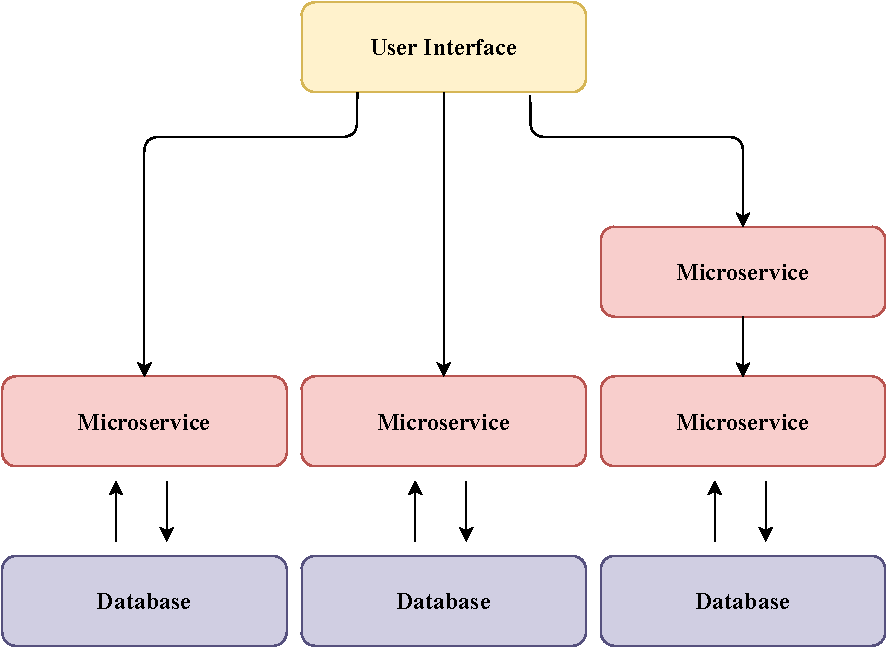
\includegraphics{../Figures/mircoservice.pdf}
    \caption{Microservices architecture}
    \label{fig:micro}
\end{figure}

\section{Comparison between Monolithic, Service-oriented and Microservices based Architectures}
Table~\ref{tbl:comp} shows the comparison between the monolithic, service-oriented and microservices based architectures based on different categories.
\begin{table}[H]
    \centering
    \begin{tabular}{|C{3.5cm}|C{3.5cm}|C{3.5cm}|C{3.5cm}|}
    \hline
    \textbf{Category}& \textbf{Monolithic}                               & \textbf{Service-oriented}& \textbf{Microservices}\\ \hline
    \textit{Type of architecture}  & Single entity                            & Centralized hub  & Decentralized \\ \hline
    \textit{Developmental complexity}     & Least                                    & Midway                            & Most complex                               \\ \hline
    \textit{Maintenance  complexity}      & Most complex                             & Easier to maintain                & Special expertise required                 \\ \hline
    \textit{Performance}                 & Most                                     & Depends on enterprise service bus & Least (can be increased with hot services) \\ \hline
    \textit{Inter-function communication} & Uses single code base                    & Uses enterprise service bus       & Uses APIs                                  \\ \hline
    \textit{Modularity}                   & None                                     & Services are modular              & Maximum                                    \\ \hline
    \textit{Use cases}                    & Simple applications with time constraint & Enterprise level applications     & Enterprise level applications              \\ \hline
    \end{tabular}
    \caption{Comparison between monolithic, service-oriented and microservices based architectures}
    \label{tbl:comp}
\end{table}
\end{document}